
\chapter{Description de l'API de \PpFf}
\label{description.chap}

\GT{Pour \'eviter la confusion, tu dois utiliser les m\^emes termes
que dans l'API, m\^eme si ces termes sont en anglais. Mais tu les mets
dans la police courrier, avec texttt.}

Ce chapitre pr\'esente l'API de \ppff. Sa conception permet aux utilisateurs de tirer parti de la simplicit\'e d'utilisation tout en cachant la complexit\'e concernant les m\'ecanismes concurrents utilis\'es. La figure~\ref{ComponentsAPI.fig} pr\'esente une vue d'ensemble de l'architecture du syst\`eme. L'API est compos\'ee de quatre \'el\'ements principaux: l'Interface avec laquelle le d\'eveloppeur interagit, les \texttt{Pipeline}s --- qui sont le coeur de l'API ---, les \texttt{Stage}s et les \texttt{Operator}s. Le r\^ole de chaque composant dans l'API est pr\'esent\'e dans la section suivante. La derni\`ere section  d\'ecrit plus en d\'etail les plus importantes m\'ethodes disponibles dans l'interface.



\begin{figure}[ht]
\centering
     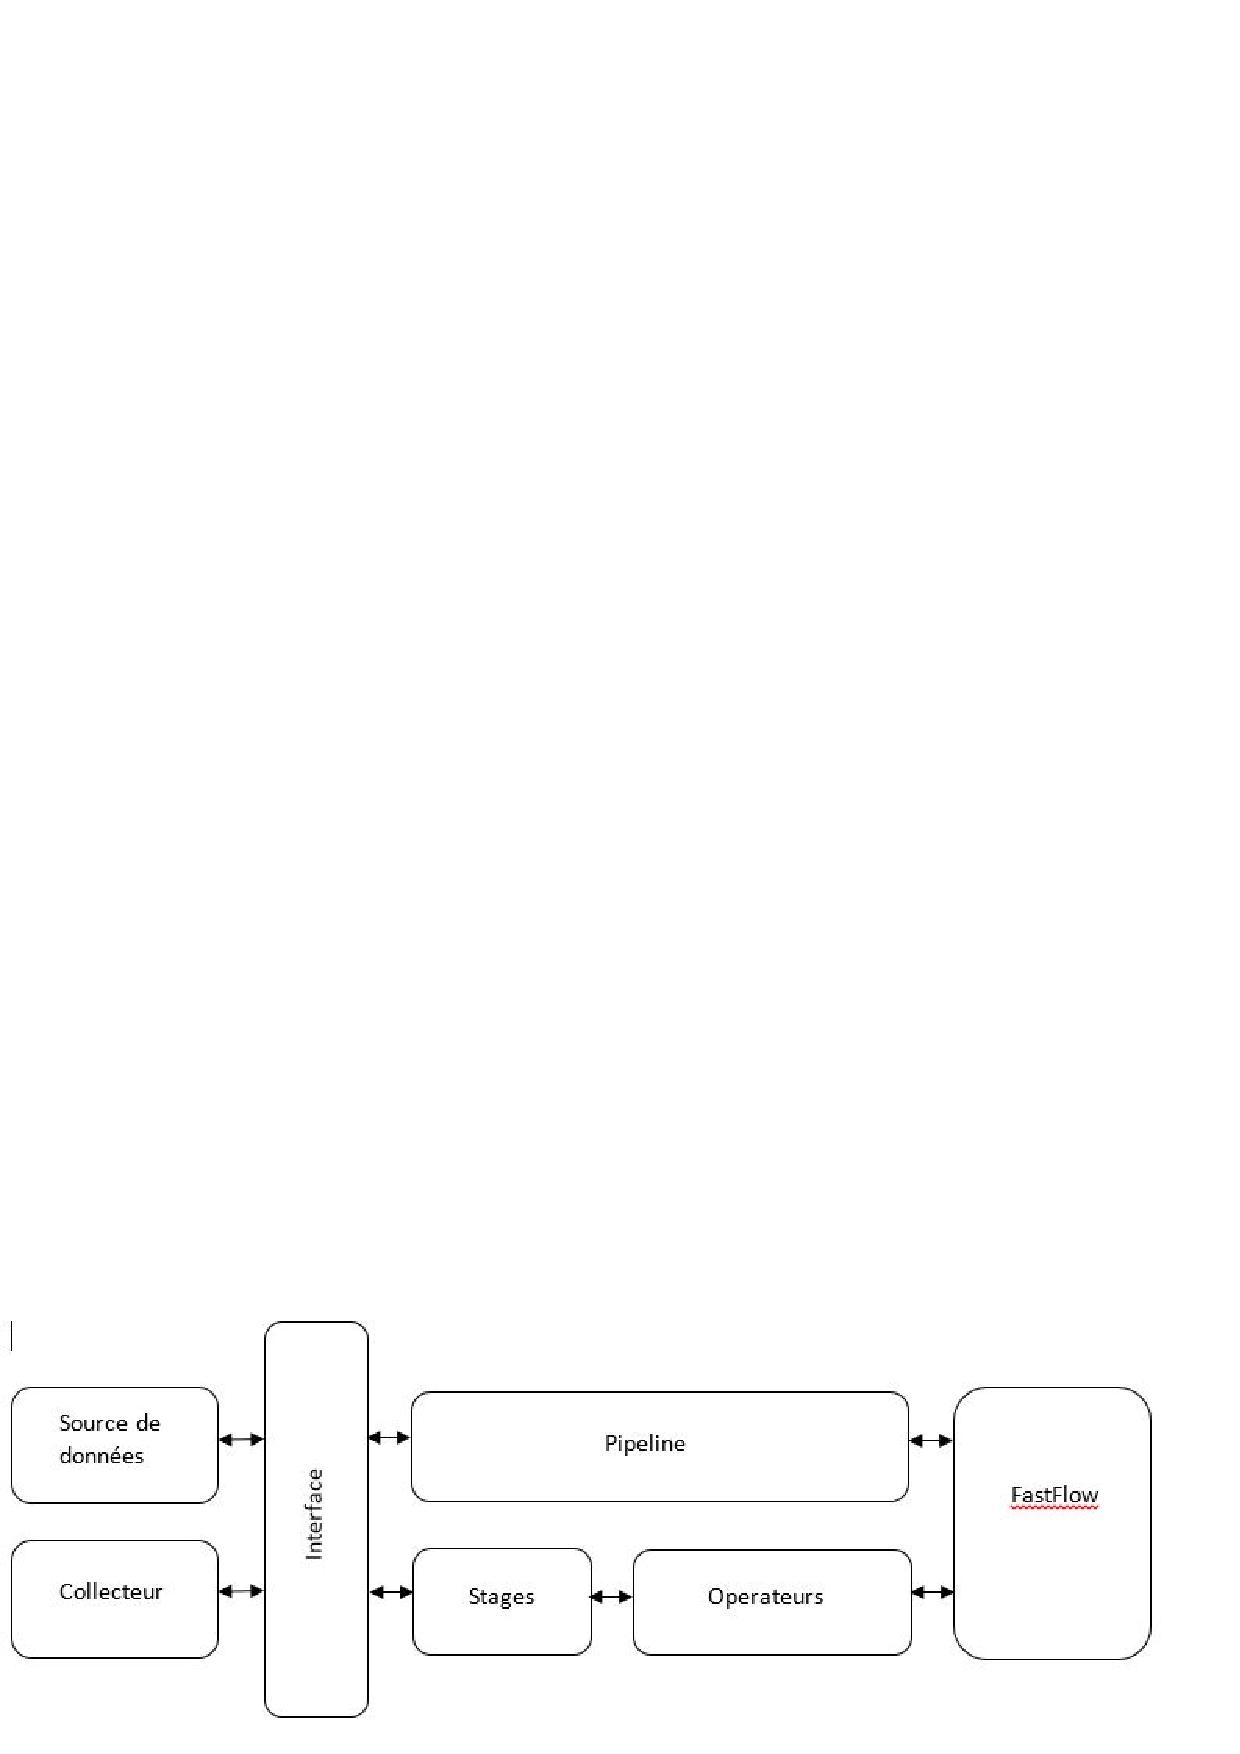
\includegraphics[width=1.0\textwidth]{Figures/ComponentsAPI.jpg}
      \caption{Composants de l'API de \ppff.}
       \label{ComponentsAPI.fig}
\end{figure}


\section{Les composants de l'API de \ppff}

\GT{Probablement qu'un diagramme de classe UML serait int\'eressant et
utile.  Il pourrait \^etre introduit ici, puis expliqu\'e dans les
sous-sections qui suivent.}

\GT{Note que de fa\c{c}on g\'en\'erale, lorsqu'on d\'ebute une section
qui contient plusieurs sous-sections, il est pr\'ef\'erable d'avoir
quelques lignes d'introduction, qui donnent une vue d'ensemble de ce
qui suit. Pas toujours, mais ici, avec le diagramme de classes, \c{c}a
ferait l'affaire.}


\subsection{Interface}

L'interface propos\'ee en PpFf consiste en un ensemble de m\'ethodes qui permettent \`a l'utilisateur de manipuler des flux de donn\'ees de mani\`ere simple et efficace. L'interface suit d'assez pr\`es celle introduite pour les \emph{Streams} de Java~8. Le tableau~\ref{methodes_api.tab} d\'ecrit bri\`evement les m\'ethodes impl\'ement\'ees dans l'API.


\GT{Dans un tabular, pour mettre du texte, on utilise p avec une
largeur. Ceci \'evite de mettre des sauts de lignes explicites, ce qui
n'est jamais une bonne id\'ee.}

\GT{Il faut mettre le code avec police tt. Par contre, j'ai essay\'e
que le code soit mis par d\'efaut ainsi, mais cela n'a pas
fonctionn\'e, d'o\`u les commandes tt ins\'er\'ees en d\'ebut de
chaque ligne~:(}

\GT{Par contre, le d\'efaut avec la solution actuelle, c'est que c'est
tr\`es difficile \`a comprendre pour les m\'ethodes plus complexes. Il
faudra qu'on r\'efl\'echisse \`a une fa\c{c}on plus claire de
pr\'esenter la signaure des m\'ethodes.}

\begin{table}[h]
\centering

\resizebox{\textwidth}{!}{%

\begin{tabular}{|l|l|p{8cm}|}
\hline
\textbf{M\'ethode} & \textbf{Type du r\'esultat} & \textbf{Description du r\'esultat}\\
\hline
	\begin{tabular}{@{}l@{}}
	\tt template<typename T> \\
	\tt allMatch(std::function<bool(T*)> predicate)
	\end{tabular} &
  	\texttt{bool} &
    Retourne \texttt{true} si tous les \'el\'ements
    de ce flux correspondent au pr\'edicat
    fourni, sinon \texttt{false}.
    \\
\hline
	\begin{tabular}{@{}l@{}}
	\tt template<typename T> \\
	\tt anyMatch(std::function<bool(T*)> predicate)
	\end{tabular} &
  	\texttt{bool} & 
    Retourne \texttt{true} si au moins un  
    \'el\'ement de ce flux correspondent
    au pr\'edicat fourni, sinon \texttt{false}.
\\
\hline
	\begin{tabular}{@{}l@{}}
	\tt template <typename T, template \\
	\tt <typename ELEM, class ALLOC = \\
	\tt std::allocator<ELEM>{}> class TContainer>\\
	\tt collect()
	\end{tabular} &
  	\texttt{TContainer<T>} &
    Retourne un conteneur de type
    STL contenant les \'el\'ements de ce flux.
    \\
\hline
	\begin{tabular}{@{}l@{}}
	\tt count()\\
	\end{tabular} &
  	\texttt{unsigned int} & 
    Retourne le nombre d'\'el\'ements
    dans ce flux.
    \\
\hline
	\begin{tabular}{@{}l@{}}
	\tt template<typename In> \\
	\tt find(std::function<bool(In*)> const\& taskFunc)
	\end{tabular} &
  	\texttt{Pipe\&} &
    Retourne tous les
    \'el\'ements du flux qui satisfont la 
    fournie en argument.
    \\
\hline
	\begin{tabular}{@{}l@{}}
	\tt template<typename In, typename Out, \\
    \tt typename OutContainer> \\
	\tt flatMap(std::function<OutContainer*(In*)> \\
    \tt const\& taskFunc)
	\end{tabular} &
  	\texttt{Pipe\&} & 
    Applique la fonction fournie en argument
    \`a chaque \'el\'ement du flux.
    \\
\hline
	\begin{tabular}{@{}l@{}}
	\tt template<typename In, typename Out, \\
    \tt typename OutContainer = In> \\
	\tt flatMap()
	\end{tabular} &
  	\texttt{Pipe\&} &
    \GT{Reformuler: je ne comprends pas la diff\'erence avec le pr\'ec\'edent}    
    \\
\hline
	\begin{tabular}{@{}l@{}}
	\tt template<typename In, typename K = In, \\
    \tt typename V = In, typename MapType> \\
	\tt groupByKey(std::function<K*(In*)> const\& \\
    \tt taskFuncOnKey, std::function<V*(In*)> \\
    \tt const\& taskFuncOnValue = identity<In,V>)
	\end{tabular} &
  	\texttt{MapType} &
    Retourne un dictionnaire (\emph{map}) avec les \'el\'ements
    du flux regroupés par cl\'e.
   \\
\hline
%	\begin{tabular}{@{}l@{}}
%	template < typename T, \\
%    template <typename ELEM, class \\
%    ALLOC = std::allocator<ELEM>> \\
%    class TContainer > \\
%	intermediateCollect()
%	\end{tabular} &
%	Collection<T, TContainer, Pipe> & \begin{tabular}{@{}l@{}}
%    Retourne une collection avec les \\
%    \'el\'ements de ce flux.
%    \end{tabular}\\ 
%\hline
%	\begin{tabular}{@{}l@{}}
%	template<typename T> \\
%	limit (int n)
%	\end{tabular} &
%	Pipe\& & \begin{tabular}{@{}l@{}}
%    Renvoie dans le flux seulement \\
%    les n premiers \'el\'ements de \\
%    ce flux.
%    \end{tabular}\\
%\hline
%	\begin{tabular}{@{}l@{}}
%	linesFromFile(const std::string\& path)
%	\end{tabular} &
%	Pipe\& & \begin{tabular}{@{}l@{}}
%    Renvoie dans le flux les lignes \\
%    contenues dans un fichier.
%    \end{tabular}\\
%\hline
%	\begin{tabular}{@{}l@{}}
%	template<typename In, typename Out> \\
%	map(std::function<Out*(In*)> const\& \\ 
%    taskFunc)m	
%	\end{tabular} &
%	Pipe\& & \begin{tabular}{@{}l@{}}
%    Renvoie dans le flux les \\
%    r\'esultats constitu\'es de \\
%    l'application d'une fonction \\
%    fournie en param\`etre aux \\
%    \'el\'ements de ce flux.
%    \end{tabular}\\
%\hline

\end{tabular}
}
\caption{Les m\'ethodes expos\'ees aux utilisateurs par l'API de \ppff.}
\label{methodes_api.tab}
\end{table}

Comme on peut le voir dans le tableau~\ref{methodes_api.tab}, la d\'eclaration des m\'ethodes utilise la programmation g\'en\'erique de C++, c'est-\`a-dire les \emph{templates}. Cela permet aux utilisateurs d'avoir une interface unique, de sorte qu'une m\'ethode peut \^etre r\'eutilis\'ee pour n'importe quel type de donn\'ees.


Un autre point cl\'e dans cette interface est son expressivit\'e. M\^eme avant sa conception d\'etaill\'ee, nous nous \'etions donn\'es comme objectif de fournir un syst\`eme suffisamment intuitif et expressif pour le traitement de flux de donn\'ees. 

\GT{Lorsque dans le texte tu indiques des identificateurs qui viennent du code --- find, collect, etc. --- alors il faut les mettre en police tt, donc \texttt{find}, \texttt{collect}, etc.}

Le pseudocode~\ref{expressivite_api.pseudo} pr\'esente un extrait de code C++ qui donne un premier aper\c{c}u de l'expressivit\'e de l'interface --- d'autres exemples seront pr\'esent\'es plus loin. Dans cet exemple, on s\'electionne les employ\'es qui ont un salaire plus grand que 35~K\$. Les employ\'es sont initialement dans un conteneur STL et sont filtr\'es en chainant trois op\'erations : $i)$ \texttt{source} qui permet d'envoyer dans le flux des objets de type \texttt{Employe}; $ii$) \texttt{find} qui s\'electionne les employ\'es selon la condition fournie en param\`etre (une lambda-expression); $iii)$ \texttt{collect} qui met les employ\'es s\'electionn\'es dans un conteneur STL. Ici, les employ\'es s\'electionn\'es sont mis dans un conteneur de type \texttt{std::vector} --- le type de conteneur est donn\'e par le type fourni en argument (g\'en\'erique) de la m\'ethode \texttt{collect}.


\begin{pseudocode}
{\small
\begin{alltt}
// Definition (omise) d'un vecteur d'objets Employe.
std::vector<Employe> sourceEmployes;
...

std::vector<Employe> result = 
        Pipe()
        .source<Employe>(sourceEmployes.begin(), sourceEmployes.end())
        .find<Employe>([](Employe *e) -> bool \{ return e->salary > 35000; \})
        .collect<Employe, std::vector>();

\end{alltt}
}
\caption{Un exemple illustrant l'\'expressivit\'e de l'API de \ppff.}
\label{expressivite_api.pseudo}
\end{pseudocode}




\subsection{Op\'erateurs}

Les op\'erateurs (\texttt{Operator}s) sont la base de notre syst\`eme. L'API fournit un ensemble d'op\'erateurs qui facilitent la t\^ache de l'utilisateur. Les op\'erateurs sont structur\'es en deux cat\'egories : les op\'erateurs sans \'etat et les op\'erateurs avec \'etat.

Les \emph{op\'erateurs sans \'etat} sont ceux qui ne disposent pas d'informations sur l'it\'eration en cours et ne transmettent pas les informations interm\'ediaires des \'etapes de traitement pr\'ec\'edentes. Si on prend comme exemple le filtre repr\'esent\'e par la m\'ethode \texttt{find} du tableau~\ref{methodes_api.tab}, il traite le flux de donn\'ees \'el\'ement par \'el\'ement. 
%
Lorsque la fonction (lambda-expression) fournie en argument \`a la m\'ethode \texttt{find} ne satisfait pas la condition lorqu'appliqu\'ee \`a un \'el\'ement du flux, le filtre ne retourne rien. Un op\'erateur sans \'etat, par contre, peut utiliser des donn\'ees historiques stock\'ees dans la m\'emoire locale ou sur le disque.

\GT{Je ne comprends pas cette derni\`ere phrase.  Si l'op\'erateur est
<<sans \'etat>>, alors il ne devrait pas non plus utiliser des
donn\'ees de la m\'emoire.  Peut-\^etre est-ce le terme <<sans
\'etat>> qui est mal chosi?}

\GT{Dans le prochain paragraphe: historique des <<op\'erations
pass\'ees>> ou des <<\'el\'ements pass\'es du flux>>?}

Les \emph{op\'erateurs avec \'etat} sont ceux qui maintiennent une structure de donn\'ees interne, qui repr\'esente l'\'etat. Cette structure pr\'eserve l'historique des op\'erations pass\'ees et affecte la logique de traitement dans les calculs ult\'erieurs. Par exemple, l'op\'erateur \texttt{Sum} calcule la somme des \'el\'ements du flux. Son \'etat contient la valeur de l'\'el\'ement en cours et la valeur de la somme de tous les \'el\'ements pr\'ec\'edents celui-ci. 


\subsection{Stages}

Le traitement du flux de donn\'ees est mod\'elis\'e en utilisant une cha\^{\i}ne d'\'etapes. Dans notre API, une \'etape est repr\'esent\'ee par un \texttt{Stage}, et chaque \texttt{Stage} est compos\'e d'un ou plusieurs op\'erateurs. Notons toutefois que ce module n'est pas visible \`a l'utilisateur. 



\subsection{Pipeline}

Le \texttt{Pipeline} est le composant principal de notre API. Un \texttt{Pipeline} est une cha\^{\i}ne de traitement compos\'ee d'un ou plusieurs \texttt{Operator}s regroup\'es dans des \texttt{Stages}. La figure~\ref{Quelle figure?} montre une vue d\'etaill\'ee d'un \texttt{Pipeline} en action. Une \'etape de la cha\^{\i}ne de traitement de ce mod\`ele traite les donn\'ees produites par l'\'etape pr\'ec\'edente dans le flux et fournit les r\'esultats \`a l'étape suivante dans le flux. Un pipeline \texttt{P} avec $n$ \'etapes peut \^etre formellement d\'efini comme suit:


\[
	\texttt{P} = O_1 + O_2 + O_3 + \ldots + O_n;
\]


Dans l'expression ci-dessus, $O_k$ d\'enote le $k^e$ op\'erateur dans le pipeline~\texttt{P}.

L'utilisation de \texttt{Pipeline} introduit une couche d'abstraction sur une cha\^{\i}ne complexe d'op\'erateurs. De plus, un \texttt{Pipeline} n'expose à l'ext\'erieur que ses entr\'ees et ses sorties. Une telle conception modulaire permet une flexibilit\'e au syst\`eme tout en simplifiant la mise en œuvre. Par exemple, le parall\'elisme du flux pourrait \^etre facilement r\'ealis\'e en ayant plusieurs \texttt{Pipeline}s identiques connect\'es \`a la m\^eme entr\'ee et sortie respectivement.


